%!TEX ROOT = thesis.tex
\chapter{THEORETICAL FRAMEWORK}
\label{chap: 3}

Chapter 3 would include a  brief history of artificial intelligence research that are directly or indirectly related to the innovation of transformers. Then, the second section would covers the foundations of deep learning which includes feed-forward neural networks, activation functions, loss functions and evaluation metric. The  section would cover the basics of transformers. The final section would include the potential challenges and limitations of this project.

\section{A Brief History of Deep Learning}

Modern deep learning as we know it today can be traced back to when Frank Rosenblatt introduced the perceptron in 1959, referring to it as the "Mark I Perceptron" shown in figure \ref{fig:perceptron}. Given an input, the perceptron will generate an output based on an activation function. The weights in the perceptron were iteratively learned by minimising the difference between the generated output and the desired output.

The perceptron never took off in popularity because it can't  learn the simple XOR function. In 1986, David Rumelhart, Geoff Hinton, and Ronald Williams showed how by incorporating "hidden" layers, a multi-layer perceptron can be used for non-linear data. Multi-layer perceptrons are also known as neural networks.

\begin{figure}[ht]
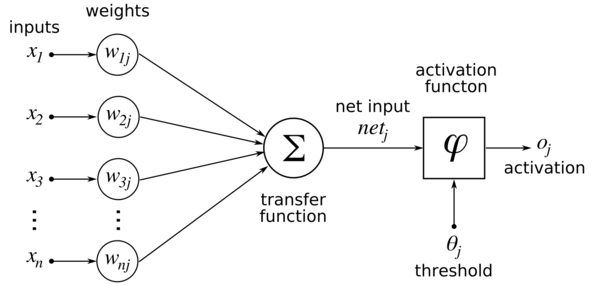
\includegraphics[width=10.5cm, height=5.5cm]{images/Rosenblattperceptron.png}
\centering
\caption{Rosenblatt Perceptron \protect\cite{markovbook}}
\label{fig:perceptron}
\end{figure}

LeCun et al., published a method to recognized hand-written digits and it was utilized by the U.S. Postal Service \cite{LeCunBoserDenkerEtAl89}, making it the first neural network model that received widesread adoption . This is a huge milestone for deep learning, proving the usefulness of convolution operations and weight learning the features in computer vision.

However, there are still a lot of flaws with neural networks. Take for example the backpropagation algorithm, has a number of issues such as vanishing gradients and the inability to learn long-term information. Hochreiter and Schmidhuber showed how  Long Short-Term Memory (LSTM) architecture could overcome the shortcomings of backpropagation.

LeCun et al. also showed the advantages of deep learning through more complex neural networks architectures such as  Deep Belief Networks (DBNs), Convolutional Neural Networks (CNNs) and Restricted Boltzmann Machines (RBMs). Li et al.,  launched ImageNet, which was the most extensive collection of labelled images and highlighted the importance of robust dataset to train a deep learning model for computer vision task. 

Mikolov et al. and Graves proposed language models using Recurrent Neural Networks (RNN) and LSTM, which later became the building blocks for many natural language processing (NLP) architectures. Sequence-to-sequence framework became the core architecture for a wide range of NLP tasks. Bahdanau et al. proposed the attention mechanism to overcome the bottleneck issue with sequence-tosequence model. Attention mechanismplays a crucial role in subsequent evolution of Transformers.

In 2017, Transformers were formally introduced in the "Attention is All You Need" paper \cite{attention-is-all-you-need} and became the most popular architecture in NLP. In 2020, Vision Transformers \cite{16x16} introduced a method to adapt Transformers for computer vision by splitting the input image into patches and represent them as vectors.

\section{Introduction to Transformers}
This section would  lays out the various building blocks of transformers such as attention, multi-head attention, positional encodings, residual connections, and encoder-decoder architecture. Subsections \ref{subsection: encoder-decoder} and \ref{subsection: sequence} would give a brief introduction to Recurrent Neural Networks (RNN) and sequence-to-sequence model (seq2seq) and the subsequent subsections would explain why attention unit and Transformers are born from RNN and seq2seq. 
\subsection{Encoder-Decoder Architecture} \label{subsection: encoder-decoder}

Because Transformers has its origin in NLP that relies on sequential input, it follows encoder-decoder architecture as shown in \ref{fig:encoder-decoder}. The encoder module takes a variable-length sequence and converts it into a fixed-length output-state while the decoder module takes a fixed-length state and converts it back into a variable-length output \cite{attention}. This approach is also known as sequence-to-sequence (seq2seq).
\FloatBarrier
\begin{figure}[ht]
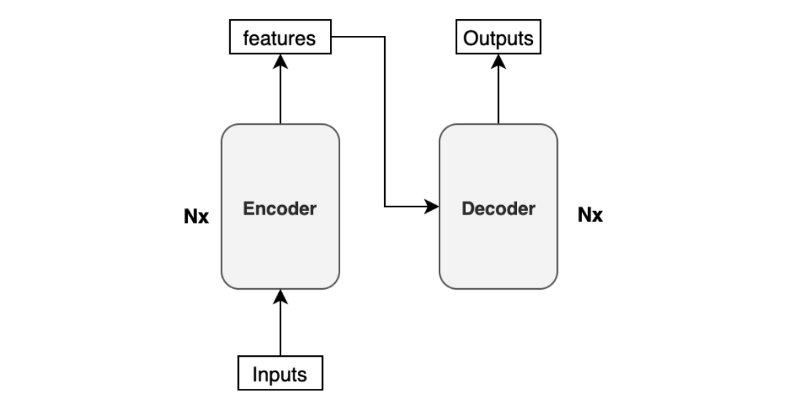
\includegraphics[width=13.5cm, height=5.5cm]{images/encodeer-decoder.jpg}
\centering
\caption{Encoder-Decoder Architecture \protect\cite{attention}}
\label{fig:encoder-decoder}
\end{figure}
\FloatBarrier


Suppose that we have an input sequence $x_1...x_t$, an embedding mapping module will transform the input sequence into vectors $\mathbf{x}_1...\mathbf{x}_t$. A unidirectional model at any time \textit{t} with a previous hidden state $\mathbf{h}_{t-1}$ and input $\mathbf{x}_t$ will generate a new hidden state:

\begin{equation}
    \mathbf{h}_t = tanh(\mathbf{Wh}_{t-1} + \mathbf{Wx}_t)
\end{equation}

\subsection{Attention Mechanism}

Attention mechanism was first introduced by \citeA{attention} and it is the most fundamental part of a Transformer which was introduced by Google in 2017 \citeA{attention-is-all-you-need}. The attention unit will take input vectors $\mathbf{x}_1...\mathbf{x}_t$ to produce output vectors $\mathbf{y}_1...\mathbf{y}_t$. $\mathbf{y}_i$ is the weighted average of all the input vectors such that:
\begin{equation}
    \mathbf{y}_i = \sum \mathbf{w}_{ij}\mathbf{x}_j
\end{equation}

Where $\mathbf{w}_{ij}$ is the dot product of $\mathbf{x}_i$ and ${x}_j$. The dot product gives us a real number so a softmax function is applied to ensure that thee output sequence sum to 1:
\begin{equation}
    w_{ij} = \frac{exp w_{ij}}{\sum_j exp w_{ij}}
\end{equation}

The self attention mechanism will use $\mathbf{x}_i$  in three different ways:
\begin{enumerate}
    \item Compare it to every other vector to obtain the \textbf{query}, \textbf{Q} which is the weights for its own output $\mathbf{y}_i$.
    \item Compare it to every other vector to obtain the \textbf{key},  \textbf{K} which is the weights for the output of the j-th vector $\mathbf{y}_j$
    \item Include it in a weighted sum to  obtain the \textbf{value},  \textbf{V}.

\end{enumerate}

Three new weight matrices are developed for each role namely: $\mathbf{W_q}, \mathbf{W_k}, \mathbf{W_v}$. These are the weights that are going to be learned by backpropagation. The dot product is scaled down as its average value grows with each added dimension $d_k$. The attention mechanism can be formally described as:
\begin{equation}
\mathbf{Q} = \mathbf{W}_q \mathbf{x}_i
\end{equation}
\begin{equation}
    \mathbf{K} = \mathbf{W}_k \mathbf{x}_i
\end{equation}
\begin{equation}
    \mathbf{V} = \mathbf{W}_v \mathbf{x}_i 
\end{equation}
\begin{equation}
    ATTENTION(\mathbf{Q,K,V}) = softmax(\frac{\mathbf{Q} \mathbf{K}^T}{\sqrt{d_k}})\mathbf{V}
\end{equation}
\begin{equation}
    \mathbf{y} = \sum ATTENTION(\mathbf{Q,K,V})\mathbf{x}    
\end{equation}

The attention mechanism is shown in figure \ref{fig:attention-unit}

\begin{figure}[ht]
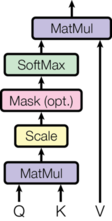
\includegraphics[width=4.0cm, height=6.5cm]{images/attention unit.png}
\centering
\caption{Illustration of Attention Mechanism Unit \protect\cite{attention-is-all-you-need}}
\label{fig:attention-unit}
\end{figure}
\FloatBarrier


\subsection{Multi Head Attention}

With the introduction of the softmax function in the previous section, we limit the attention value to either 0 or 1 when in reality attention can be anywhere in between. This is a negative consequence of using the softmax function. The easiest solution is to have multiple attention heads running at once. The multi-attention head is shown in figure \ref{fig:multi-head}.

\begin{figure}[ht]
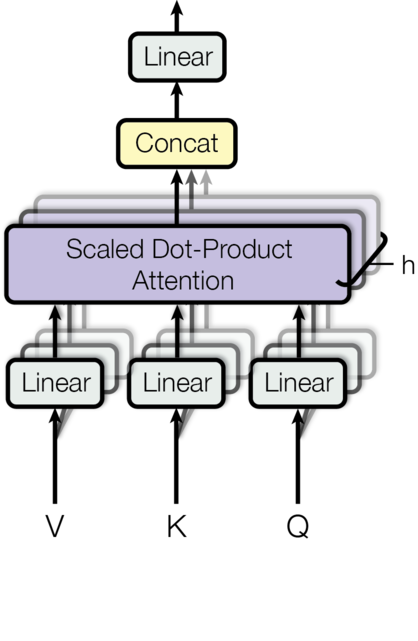
\includegraphics[width=5.5cm, height=7.5cm]{images/multi-head attention.png}
\centering
\caption{Illustration of Multi-head Attention \protect\cite{attention-is-all-you-need}}
\label{fig:multi-head}
\end{figure}
\FloatBarrier

Multi-attention head is a set of the self-attention mechanism running in parallel. However, generating $\mathbf{K}$, $\mathbf{Q}$ and $\mathbf{V}$ for each head would be computationally expensive. We avoid this problem by scaling it down by a factor of the square root of the number of headsas shown in \citeA{attention-is-all-you-need}. The entire with multi-head attention module is shown in figure \ref{fig:transformer-architecture}

\FloatBarrier
\begin{figure}[ht]
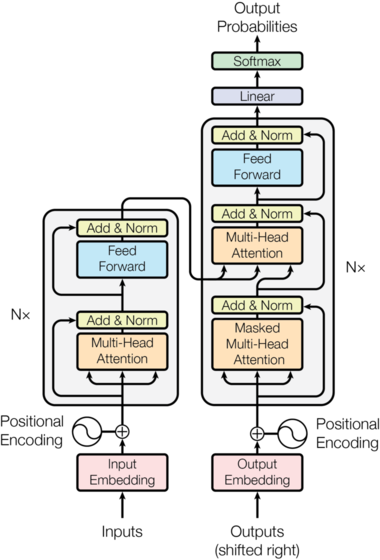
\includegraphics[width=6.5cm, height=9.5cm]{images/transformer_architecture.png}
\centering
\caption{Illustration of Transformer Architecture \protect\cite{attention-is-all-you-need}}
\label{fig:transformer-architecture}
\end{figure}
\FloatBarrier

\section{Activation Functions}
This section contains the three most commonly used activation functions in deep learning, the sigmoid function, the ReLU function and the softmax function.
\subsection{Sigmoid Function}
Sigmoid function is a special form of the logistic function that would map any real numbered input to either 0 or 1 and is given by:
\begin{equation}
    \sigma (x) = \frac{1}{1+exp(-x)}
\end{equation}

Figure \ref{fig: sigmoid} shows a plot of the sigmoid function.
\FloatBarrier
\begin{figure}[ht]
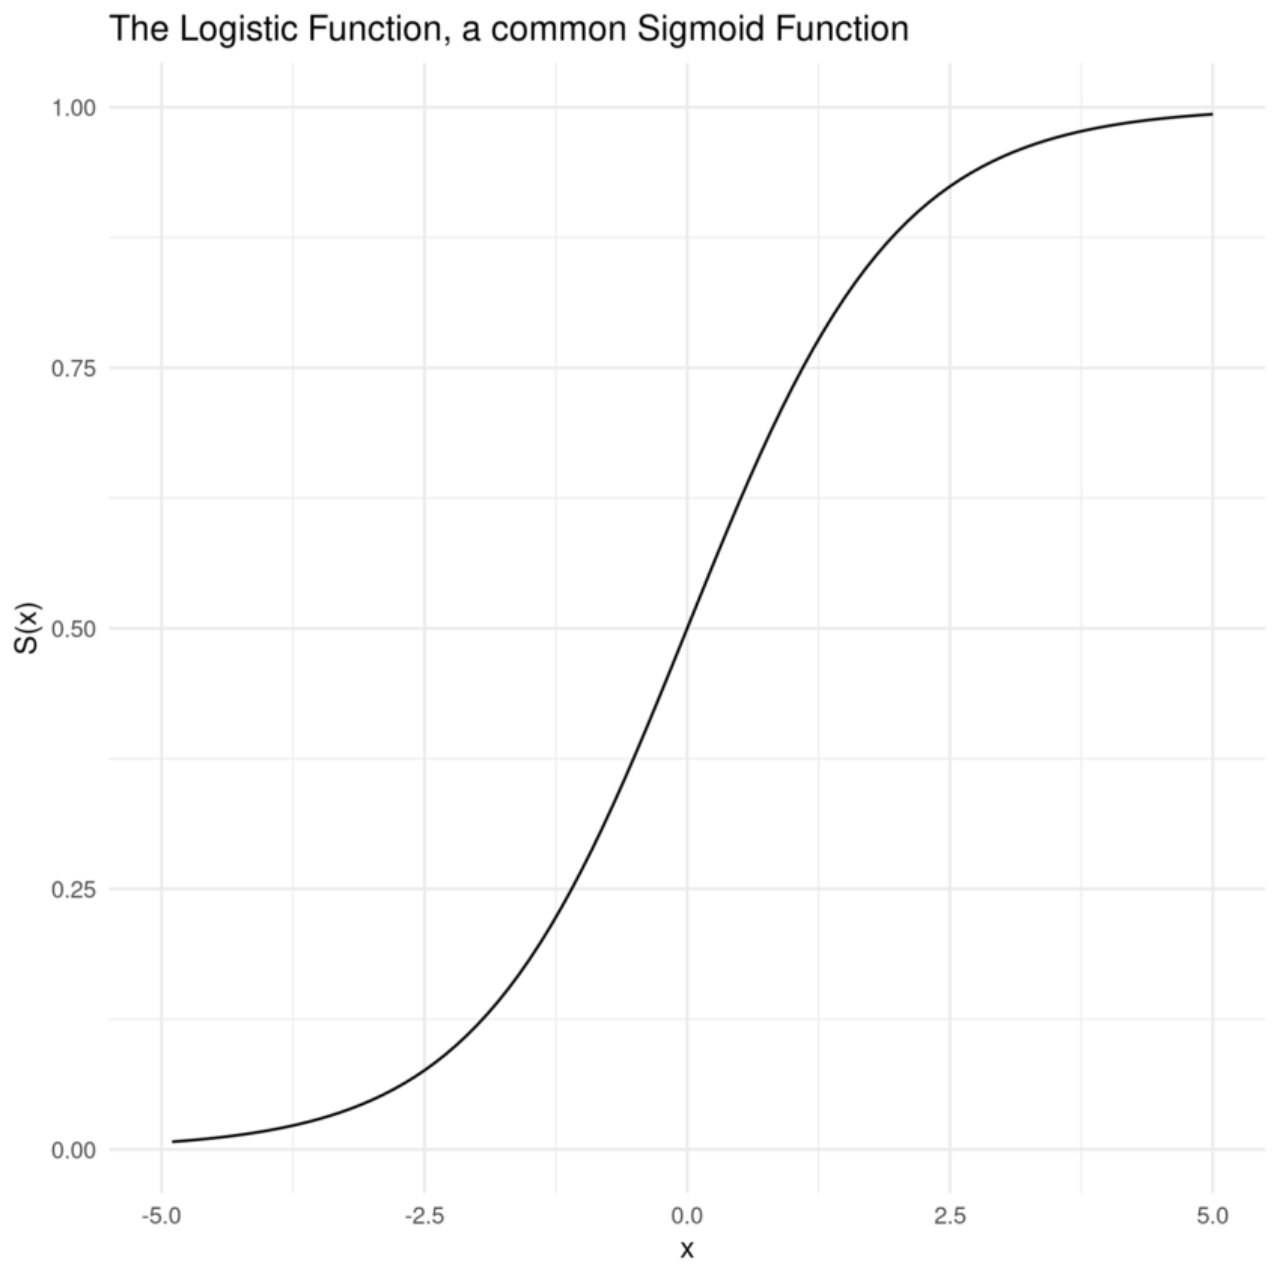
\includegraphics[width=7.5cm, height=6.5cm]{images/sigmoid.jpg}
\centering
\caption{Sigmoid Function}
\label{fig:sigmoid}
\end{figure}
\FloatBarrier


\subsection{Rectified Linear Unit Function}

There are several issues when we use sigmoid function for deep learning. The first issue is the function is only really sensitive to changes around its mid-point of its input. The second issue is that sigmoid function is computationally intensive. In order to use optimization technique such as SGD or ADAM with backpropagation to train deep neural networks, a non-linear activation function that behaves like a linear function is needed. The function must also be more sensitive to changes in the input.

Rectified Linear Unit (ReLU) function returns the input value directly, or the value 0 if the input is 0 or less. Figure \ref{fig:relu} shows a plot of the ReLU function. ReLu function can be written as:
\begin{equation}
    f(x) = max(0,x)
\end{equation}

\begin{figure}[ht]
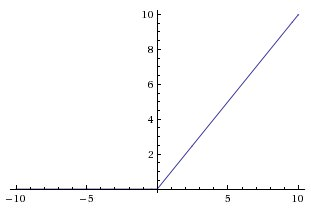
\includegraphics[width=7.5cm, height=6.5cm]{images/relu.jpeg}
\centering
\caption{ReLU Function}
\label{fig:relu}
\end{figure}
\FloatBarrier

\subsection{Softmax Function}

The softmax function produces a vector of K real values that add to 1 from a vector of K real values. The input values can be any real numbers, and softmax will translate them into probabilities by mapping them to values between 0 and 1 and can be written as follows:
\begin{equation}
    \sigma(z) = \frac{e^{z_i}}{\sum_{j=1}^K e^{z_j}}
\end{equation}

where $z_i$ is an element of the input vector and the denominator is the sum of the input vector.

\section{Backpropagation}

The goal of backpropagation is to compute the partial derivative of the cost function $C$ with respect to weights $w$ , $\frac{\partial C}{\partial w}$ and   the partial derivative of the cost function $C$ with respect to bias $b$, $\frac{\partial C}{\partial b}$, The cost function $C$ can be expressed as:
\begin{equation}
    C(X,\theta) = \frac{1}{2n} \sum_x ||\hat{y}(x) - y(x)||^2 
\end{equation}

Where $n$ is the total number of training examples, $x$ ias the input, $\hat{y}(x)$ is the desired output; and $y(x)$ is actual outputs. At each iteration, the weights and biases (collectively denoted as $\theta$) is updated according to the learning rate, $\alpha$ as follows:
\begin{equation}
    \theta^{t+1} = \theta^t - \alpha \frac{\partial C(X,\theta^t)}{\partial \theta}
\end{equation}
where $\theta^t$ is the weights and biases of the network and $t$ is the iteration value.

The derivative can be determined with respect to each input-output pair separately and combined at the end since $C$ can be decomposed into a sum over individual error terms for each distinct input-output pair:
\begin{equation}
    \frac{\partial C(X,\theta)}{\partial w_{ij}^k} = \frac{1}{N} \sum_x \frac{\partial}{\partial w_{ij}^k}(\frac{1}{2}(\hat{y}_d-y_d)^2) = \frac{1}{N} \sum_x \frac{\partial C_d}{\partial w_{ij}^k}
\end{equation}

Lastly, the weights are updated as follows:
\begin{equation}
    \Delta w_{ij}^k = - \alpha \frac{\partial C(X,\theta)}{\partial w_{ij}^k}
\end{equation}

\subsection{Swin Transformer}
The first version of Swin Transformer \cite{swin-v1} presents a hierarchical feature representation. It delivered great performances with linear computational complexity, which makes it suitable for semantic segmentation. Just like in ViT, Swin Transformer will use patch embedding to the input image but the difference now is the patch size is 4x4x3 instead of 16x16x3. The biggest difference between ViT and Swin Transformer is ViT attention layers work on the entire image while Swin Transformer will first compute attention on local windows. Take an example in figure \ref{fig:swin-vs-vit}, the input image is 64x64 and Swin Transformer will first use 16 non-overlapping local windows to divide the image into 16 patches. As self-attention is computed at local window, they only handle the relationships between 16 image patches. At the next level, Swin Transformer merges neighboring patches to form 4 new local windows. Therefore, those layers only deal with 16 feature patches hence maintaining the number of patches at every level. Eventually, one local window covers the entire image with 16 feature patches.
\FloatBarrier
\begin{figure}[ht]
\centering
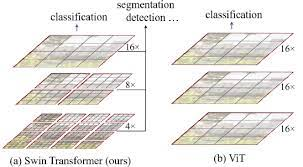
\includegraphics[width=9.5cm, height=5.5cm]{images/swin vs vit.png}
\caption{The difference between Swin Transformer and ViT \protect\cite{swin-v1}}
\label{fig:swin-vs-vit}
\end{figure}
\FloatBarrier

Swin Transformer is made up of 4 stages as shown in \ref{fig:swin architecture1}. The iinput image comes in a dimension of H x W x 3 where H and W are the height and width of the image . Swin Transformer uses a patch size of 4x4 which will produce H/4 x W/4 number of patches, and each patch’s feature dimension is 48 (4 x 4 x 3). In stage 1, the linear layer transforms the raw features to an arbitrary dimension $C$.

In stage 2, the patch merging layer concatenates the features of each group of 2 x 2 neighboring patches. Each patch’s feature dimension becomes 4C, on which it applies a linear layer, reducing the output dimension to 2C. So, we have H/8 x W/8 patches, each of which has 2C-dimensional features. The same processes are repeated in stages 3 and 4, reducing the size by 4 and increasing the feature dimension by 2.

\FloatBarrier
\begin{figure}[ht]
\centering
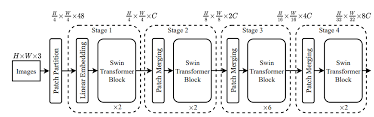
\includegraphics[width=11.5cm, height=4.5cm]{images/swin-transformer-4block.png}
\caption{Swin Transformer V1 Architecture \protect\cite{swin-v1}}
\label{fig:swin architecture1}
\end{figure}

Swin Transformer introduced a Shifted Window Multi-headed Self-Attention (W-MSA) which is an improvement of the original Multi-Headed Self Attention (MSA) to make the self-attention linear to the number of tokens. The computational complexity of the MSA is:
\begin{equation}
    \Omega (\mathbf{MSA}) = 4hwC^2 + 2(hw)^2C
\end{equation}
Where $h$ is the height of the patch, $w$ is the width of the patch and $C$ is the feature size. While the improved computational complexity of W-MSA is linis:
\begin{equation}
    \Omega (\mathbf{W-MSA}) = 4hwC^2 + 2M^2hwC
\end{equation}

Swin Transformer alternates between two partitioning configurations in consecutive Swin Transformer blocks. As shown figure \ref{fig:swin shifted}, layer 1 uses regular partitioning while layer 2 uses a windowing configuration shifted by half of the window size. They introduces connections between neighboring windows while keeping the local computation within each non-overlapping window.

The main issue with this approach is the number of local windows increased from 4 to 9. For this reason, Swin Transformer uses another mechanism called cyclic shifting. Cyclic shifting shift the image patches toward the top-left direction and then applies a mask to limit self-attention within adjacent patches. It also utilizes reverse cyclic shifting to cover the other areas. Cyclic shifting is shown in figure \ref{fig:swin cyclic}
\begin{figure}[ht]
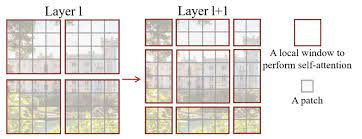
\includegraphics[width=10.5cm, height=4.5cm]{images/swin-msa1.jpeg}
\centering
\caption{Shifted Window Multi-head Self-Attention \protect\cite{swin-v1}}
\label{fig:swin shifted}
\end{figure}

\begin{figure}[ht]
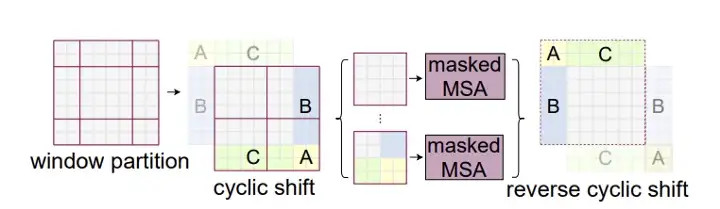
\includegraphics[width=13.5cm, height=5.5cm]{images/swin-cyclic-shift.jpg}
\centering
\caption{Cyclic Shifted Windows in Swin Transformer \protect\cite{swin-v1}}
\label{fig:swin cyclic}
\end{figure}

\FloatBarrier

SW-MSA successfully introduced connections between windows while masking prevents the attention computation from processing across the image boundary. Figure \ref{fig:2swins} show two consecutive Swin Transformer blocks with each one having a different partitioning scheme.
\FloatBarrier
\begin{figure}[ht]
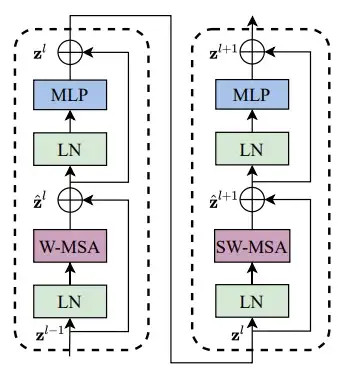
\includegraphics[width=6.5cm, height=7cm]{images/swin-architecture.jpg}
\centering
\caption{Two Successive Swin Transformer Blocks \protect\cite{swin-v1}}
\label{fig:2swins}
\end{figure}

The self-attention score using SW-MSA can be calculated as follows:
\begin{equation}
    Attention(Q,K,V) = softmax(\frac{QK^T}{\sqrt{d}+B})V
\end{equation}

Swin Transformer V2 \cite{swin-v2} was introduced in 2021 and it is an improved version of Swin Transformer to increase scalability, accuracy and stability during training. As shown in figure \ref{fig:swin v1 vs v2}, the Layer Normalization block is moved from front to back of the residual unit and a new scaled cosine self-attention unit is used in place of the old matrix multiplication based self-attention. The new self-attention score can be expressed as:
\begin{equation}
    Sim(\mathbf{q}_i,\mathbf{k}_j) = \frac{cos(\mathbf{q}_i,\mathbf{k}_j)}{\tau} + B_{ij}
\end{equation}

Where $B_{ij}$ is the relative position bias between pixel i and j; $\tau$ is a learnable scalar that is set larger than 0.01. These approaches make the model insensitive to the magnitude (largeness) of activations.
\FloatBarrier
\begin{figure}[ht]
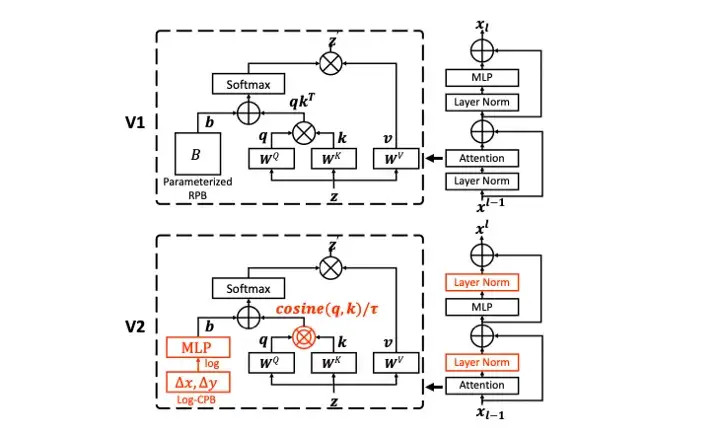
\includegraphics[width=13.5cm, height=9.5cm]{images/swin1-vs-swin2.jpg}
\centering
\caption{Difference Between Swin V1 and Swin V2 \protect\cite{swin-v2}}
\label{fig:swin v1 vs v2}
\end{figure}
\FloatBarrier

\section{Pruning Vision Transformer}

Pruning a deep learning model is a technique to reduce the number of its parameters by removing redundant values. This would allow us to deploy the model and guarantee that it would run smoothly on every device. This section would discuss several techniques to prune a Vision Transformer.

Pruning can be divided into two schemes, structured pruning and unstructured pruning. Structural pruning alters the structure of the network by physically removing grouped parameters, while unstructured pruning remove the redundant weights after the training is finished without any modification to the network \cite{depgraph}. Unstructured pruning are easier to deploy as it does not relies on specific techniques, thereby making it more popular.

An example of unstructured pruning is to set a minimum threshold of weight at the end of a layer and any values that is smaller than that threshold will be change to zero. This method would be easily done using torch.nn.utils.prune package provided by Pytorch however it greatly decrease the performance of the model. We will need a more comprehensive and systematic approach to prune our Vision Transformer.

Structured pruning is a challenging task deep neural networks are made up of a large number of basic modules like convolution, normalization, or attention, that are intrinsically connected. As an example, if we seek to remove only one layer from a Transformer, we have to inevitably take care of its inter-
dependencies to all layers simultaneously, otherwise we will end up with a broken network.

The first comprehensive method to prune a Vision Transformer is to learn its associated importance score before pruning its parameters \cite{pruning-vit}. For the features $x \in \mathbb{R}^{n \times d}$ , where $n$ is the number of features that we want to prune and $d$ is the dimension of each feature, the proposed method will preserve the generated important features and remove the useless ones. Suppose the optimal importance score is $a^* \in \mathbb{R}^d$. This method is applied on DeiT-base \cite{deit} trained on ImageNet-1k and ImageNet 100. 
\citeA{pruning-block} identified that there are three ways to compress a model. The first method is distillation which produces smaller models with a dense structure. Distillation has been proven successful in language models such as DistilBERT \cite{distilbert} and TinyBERT \cite{tinybert} which are all compressed versions of BERT \cite{bert}. The second method is pruning and third method is a combination of pruning and distillation. Distillation requires a very tedious engineering process and it is very hard to achieve.

\citeA{pruning-block} also categorized pruning into three methods. The first one being the score-based pruning methods \cite{score-pruning} replace the original parameter matrices with a masked version by adding score parameters \textbf{S} for each parameter i. The simplest one would be to zero-out the parameters with the lowest value as discussed earlier. The second pruning technique is movement pruning, which pushes the model to refine its parameters while reducing the scores of irrelevant parameters and promoting sparsity.

The third pruning method is block movement pruning \cite{pruning-block} which is a hybrid of movement and block pruning that divides each Transformer matrix into a number of fixed-sized blocks. Each block would be given a new mask and behave as a separate group in the regularisation with a common score parameter. This method has not been used alongside a Vision Transformer but they did use it to train BERT \cite{bert}, a Transformer language model with 110M parameters for question answering and sentence classification. Overall, they managed to reduce the number of parameters by a factor of 5.91 and trained it $2.24$ times faster with only a 1.99\% drop in F1 score.

